\documentclass[a4paper]{report}
\usepackage[utf8]{inputenc}
\usepackage[T1]{fontenc}
\usepackage[cache=false]{minted}
\usepackage[dvipsnames]{xcolor}
\usepackage{a4wide,syntax,listings,appendix,amsmath,tikz,wrapfig,graphicx,hyperref,pdflscape}
\hypersetup{pdftitle={Processing an Angolan Newspaper},
pdfauthor={Pedro Mendes},
colorlinks=true,
urlcolor=blue,
linkcolor=black}
\usetikzlibrary{arrows,positioning,automata,decorations.markings,shadows,shapes,calc}

\begin{document}

\title{Informatics Dictionary}
\author{Pedro Mendes (a79003)}
\date{\today}

\begin{center}
    \begin{minipage}{0.75\linewidth}
        \centering
        
\includegraphics[width=0.4\textwidth]{eng.jpeg}\par\vspace{1cm}
        \vspace{1.5cm}
        \href{https://www.uminho.pt/PT}
        {\color{black}{\scshape\LARGE Universidade do Minho}} \par
        \vspace{1cm}
        \href{https://www.di.uminho.pt/}
        {\color{black}{\scshape\Large Departamento de Informática}} \par
        \vspace{1.5cm}
        \maketitle
    \end{minipage}
\end{center}

\begin{abstract}
    \begin{center}
    \end{center}
\end{abstract}

\tableofcontents

\pagebreak

\chapter{Introduction}

This project aims to create a simple and intuitive language to describe a
dictionary and later annotate texts with.

First we'll analyse the problem, see what needs to be implemented and what
challenges need to be overcome to implement said features.

Next we'll look at the solutions to the proposed problems, dedicating a
section to the solution of each problem.
% TODO: FINISH THIS

\chapter{Problem}

The problem this program intends to solve is the following, the informatics
department wants to create a dictionary of commonly used words, associating
with each of them a \textit{meaning}, the \textit{English name} and a list of
\textit{synonyms}. This dictionary is read in conjunction with texts (that may
or may not contain a title) and annotates them with footnotes explaining the
words that are defined in the dictionary.

To solve this problem, a DSL\footnote{Domain Specific Language} needs to be
defined where the dictionary can be stored as well as texts to annotate. It's
also important that the language is user friendly as it is intended to be
human readable and writeable.

\chapter{Solution}\label{cha:solution}

\section{Definition of the SATI language}

Similarly to how an imperative
program is split in two, declarations and instructions, this language is split
between dictionary (\textit{Dicl}) and texts (\textit{Texts}), separated by one or more `\verb!\%!'.

\begin{grammar}
    <sati> $\to$ <dicl> '\%' <texts>
\end{grammar}

\subsection{Dictionary}

The dictionary is a collection of words and each word is composed of 4 parts.

\begin{grammar}
    <dicl> $\to$ <word>
    \alt <dicl> <word>
\end{grammar}

The word to find in the dictionary \textit{WD}, it's meaning \textit{Meaning}
the \textit{English Name} and finally either a list of synonyms or a single
synonym.

The list of synonyms contains synonyms separated by \verb!','! and the last one
on the list may or may not be followed by a comma.

\begin{grammar}
    <word> $\to$ <wd> `:' <meaning> `|' <englishName> `|' `[' <synonyms> `]' `;'
    \alt <meaning> `|' <englishName> `|' <synonym> `;'

    <synonyms> $\to$ <synonym> `,'
    \alt <synonyms> <synonym> `,'
    \alt <synonyms> <synonym>

    <wd> $\to$ <ID>

    <meaning> $\to$ <ID>

    <englishName> $\to$ <ID>

    <synonym> $\to$ <ID>
\end{grammar}

As an example, a dictionary can be written like this:

\begin{verbatim}
Encapsulamento : Um mecanismo da linguagem para
                 restringir o acesso aos componentes
                 de um objecto.
               | Encapsulation | Modularidade
               ;

Imutabilidade : Uma propriedade de informação que
                implica que esta não pode ser alterada.
              | Imutability
              | [ Constante, Inalteravel, ]
              ;
\end{verbatim}

\section{Texts}\label{sec:texts}

The texts section is composed of texts that may or may not have a title, the
title is used to name the \LaTeX chapter, if no title is given then
\textit{Untitled X} will be used where \textit{X} is the number of untitled
texts parsed so far.

The texts are surrounded by double quotes \verb!"! and their title is text
preceding the text. The language specification for presenting the texts is the
following:

\begin{grammar}
    <texts> $\to$ `\"' <text> `\"'
    \alt <texts> `\"' <text> `\"'
    \alt <texts> <title> `\"' <text> `\"'
    \alt <title> `\"' <text> `\"'

    <text> $\to$ <TEXT>

    <title> $\to$ <TEXT>
\end{grammar}

And a sample text section could be:

\begin{verbatim}
POO "O encapsulamento permite uma maior modularidade e organização do código."
"Em programação é muito importante o single responsability principle."
\end{verbatim}

\begin{landscape}
    \begin{figure}[p]
        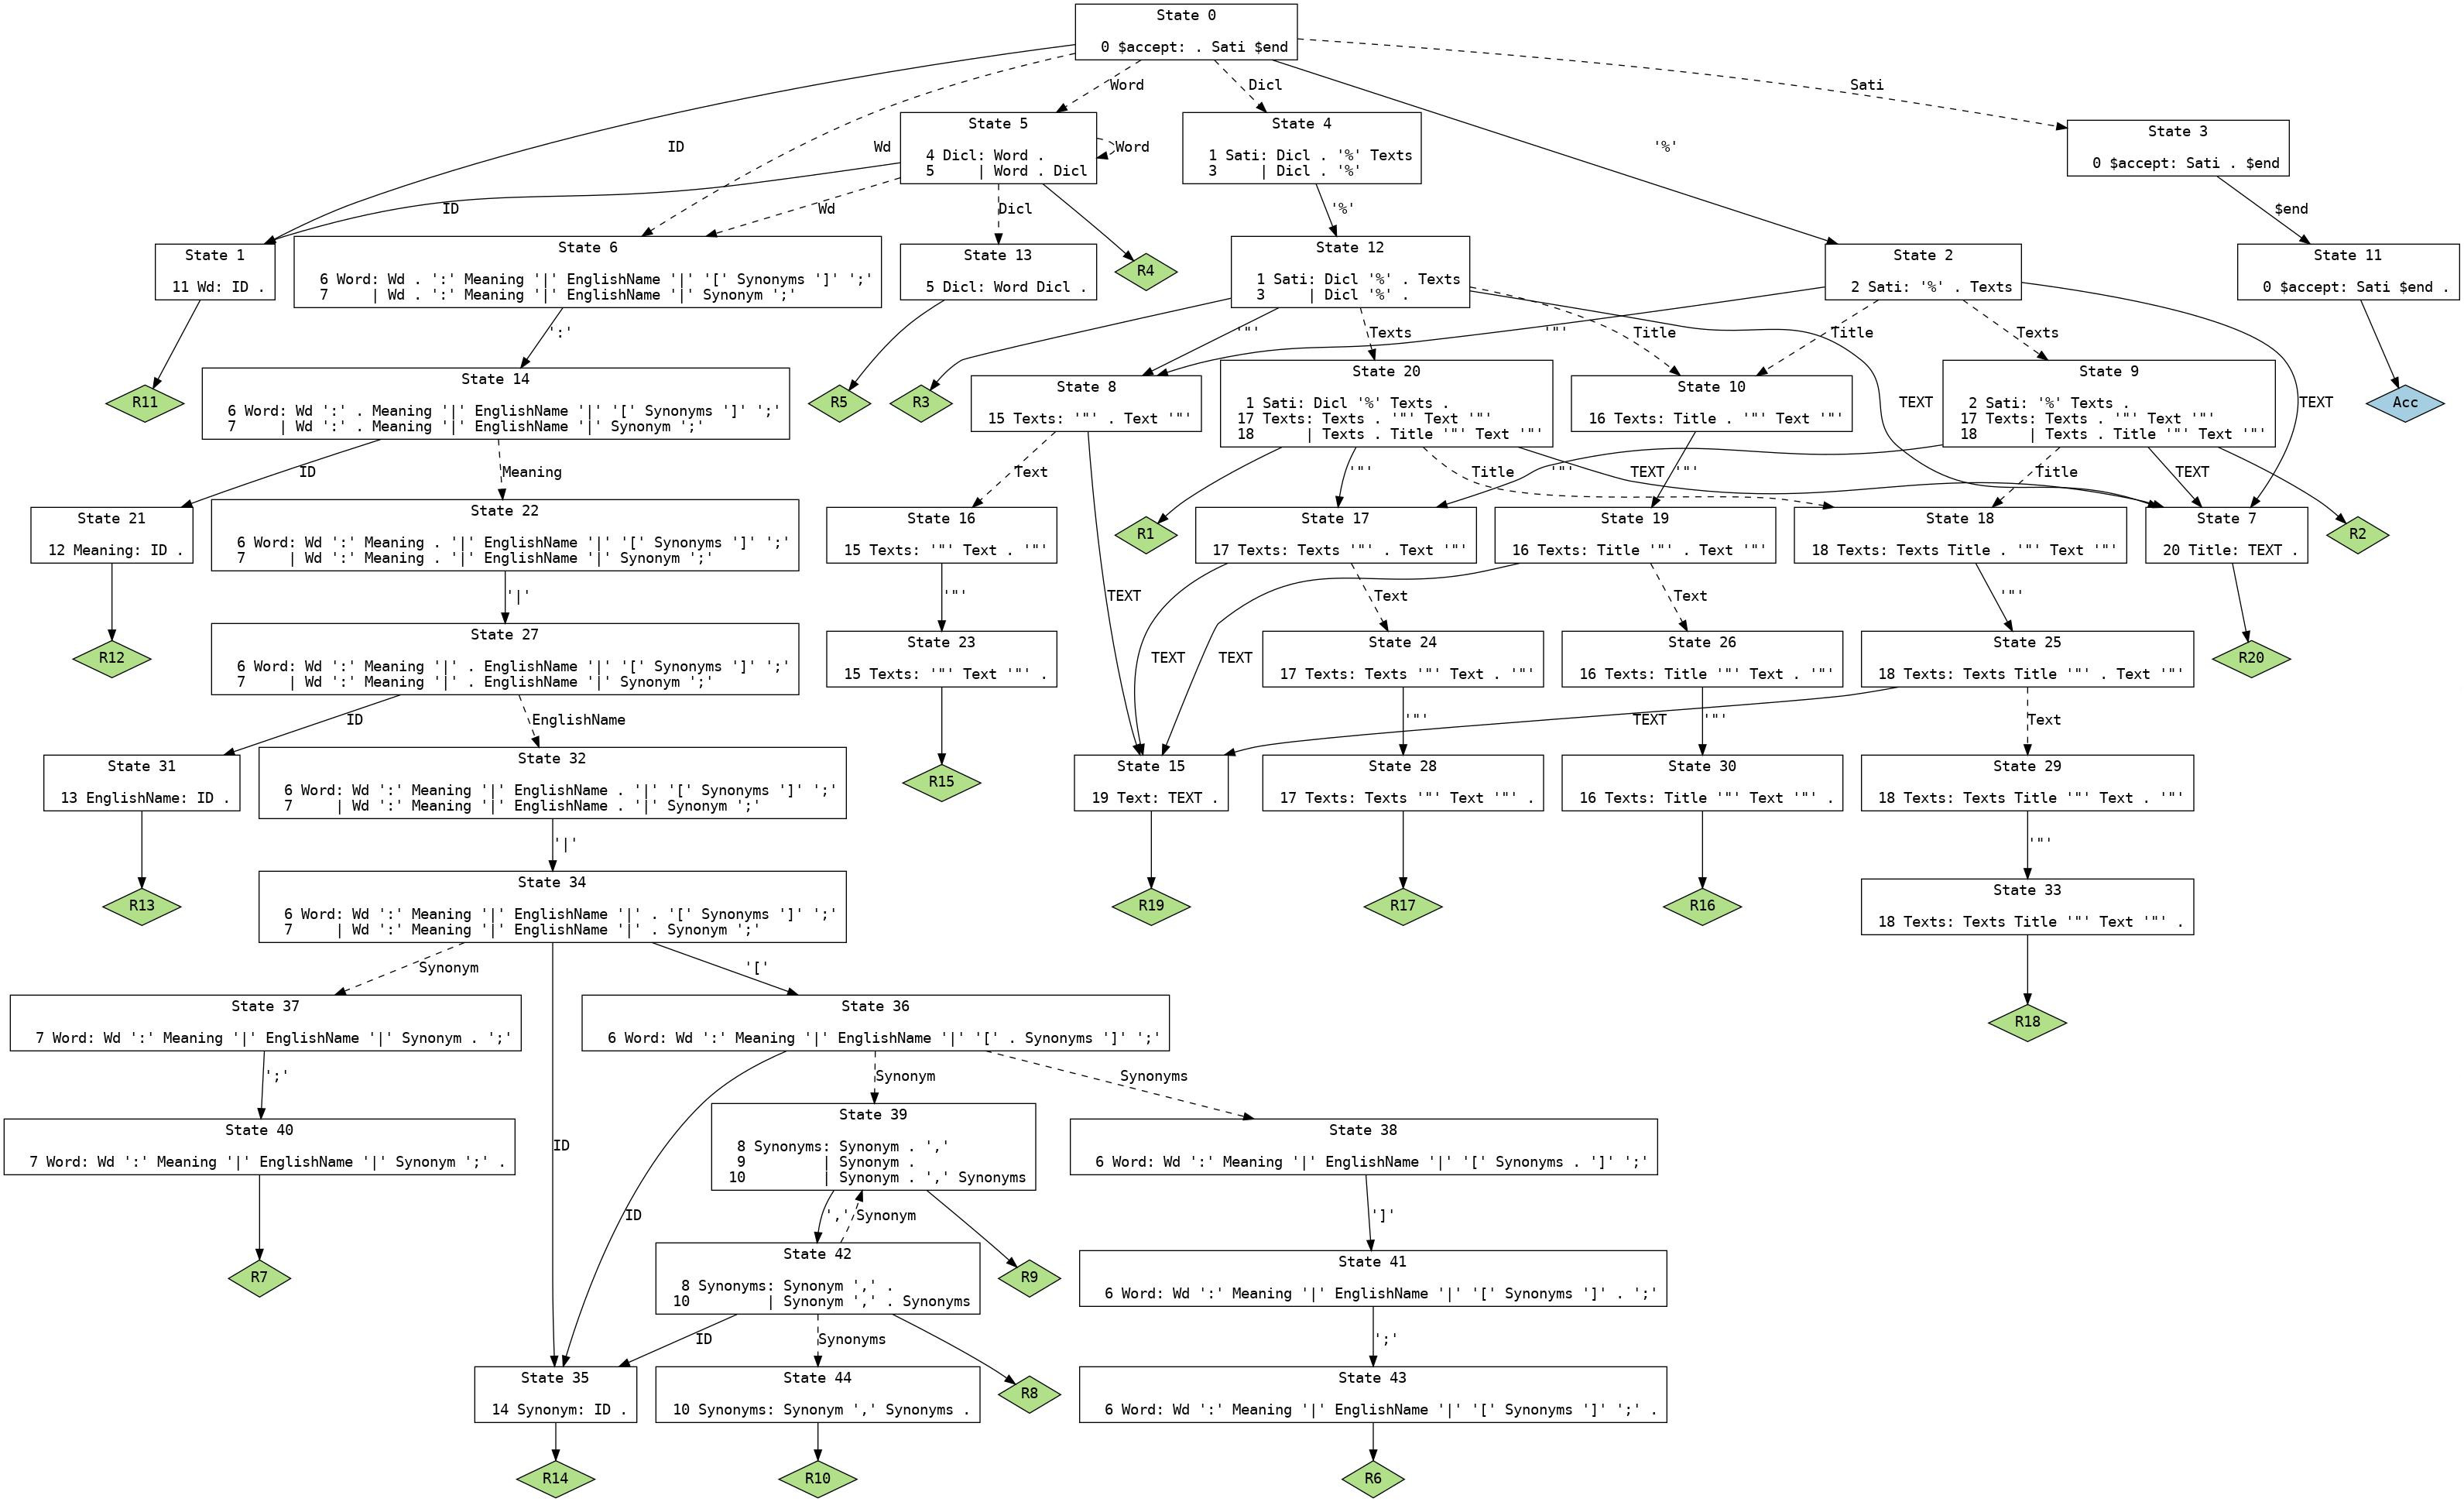
\includegraphics[height=\textwidth]{./sati.jpg}
        \caption{The Parser's Automata generated by \textit{yacc}}
    \end{figure}
\end{landscape}

And the full SATI file can be something like this.

\begin{verbatim}
Encapsulamento : Um mecanismo da linguagem para
                 restringir o acesso aos componentes
                 de um objecto.
               | Encapsulation
               | Modularidade
               ;

Imutabilidade : Uma propriedade de informação que
                implica que esta não pode ser alterada.
              | Imutability
              | [ Constante, Inalteravel, ]
              ;
%%
POO "O encapsulamento permite uma maior modularidade e organização do código."
"Em programação é muito importante o single responsability principle."
\end{verbatim}

\subsection{Lexing}

To obtain all the literals and terminal tokens (\texttt{ID} and \texttt{TEXT})
a lexer was written in \textit{flex}. Here the same two zones (\textit{Dicl}
and \textit{Texts}) were used, where \textit{Dicl} is the \texttt{INITIAL}
state and \textit{Texts} is \texttt{TEXTS} state. When the sequence of `\%' is
found the lexer switches state and returns the `\%'. In this manner we can see
what characters can not be part of each of the terminal symbols. For the
\texttt{ID} we see that the symbols \verb!% ; , " [ ] : |! cannot be used. And
for \texttt{TEXT} `\verb!"!' cannot be used, the latter can be fixed by
replacing all `\verb!"!' with `\verb!``!', as \LaTeX interprets these as double
quotes.

\lstinputlisting[firstline=7,lastline=17,basicstyle=\footnotesize\ttfamily]
{../src/sati.l}

\section{Architecture}

The architecture is split in two parts, the parsing of the dictionary and the
parsing mutation of the input texts.

\begin{wrapfigure}{r}{5.5cm}
    \centering
    \tikzstyle{struct}=[fill=white, draw=black, rectangle split, drop shadow, rectangle split parts=2]
\newcommand{\type}[1]{\textcolor{BurntOrange}{#1}}
\begin{tikzpicture}[font=\ttfamily,auto]
    \node (Sati) [struct]{%
        \nodepart[text centered, text=MidnightBlue]{one}\textbf{Sati}
        \nodepart[text width=5.3cm]{second}
        dictionary: \type{Map}<\type{String}, \type{Word}>\newline
        current\_word: \type{String}\newline
        untitled\_number: \type{int}\newline
        output: \type{File}*
        };
    \node (Word) [struct, below = of Sati]{%
        \nodepart[text centered, text=MidnightBlue]{one}\textbf{Word}
        \nodepart[text width=3.7cm]{second}
        wd: \type{String}\newline
        meaning: \type{String}\newline
        english\_name: \type{String}\newline
        synonyms: [\type{String}]
        };
\end{tikzpicture}

    \caption{Structures}
\end{wrapfigure}

To achieve this, the following structures were designed: A word struct
that represents each word in the dictionary, and the main \texttt{Sati} struct
that stores the dictionary as well as some extra information.

The \texttt{Word} struct is pretty self-explanatory. It contains the same fields
as the ones described by the language. The word itself, its meaning, the
English name, and a list of synonyms.

The \texttt{Sati} struct is a bit more complex. First and foremost it has a
\texttt{dictionary} that stores the \texttt{Word}s associated with the word
(String). Then it has the \texttt{current\_word} field, (this will be
explained more in depth in SubSection~\ref{ssec:parsing-the-dict}), but it
keeps track of the word that is being currently parsed. Next comes the
\texttt{untitled\_number}, this serves to count the number of untitled posts in
order to produce the behaviour described in Section~\ref{sec:texts}. And
finally, the \texttt{output} field, which stores the file where to output the
content, this is the standard output, by default, but can be changed with the
flags documented in Chapter~\ref{cha:flags}.

\subsection{Parsing the dictionary}\label{ssec:parsing-the-dict}

To parse the dictionary 2 elements of the \texttt{Sait} struct are used, the
\texttt{dictionary} and the \texttt{current\_word}, when a new word is added
it's added to the \texttt{dictionary} and the key is stored in
\texttt{current\_word}, then, when a meaning, English name or synonym is added
the \texttt{current\_word} is used to access the \texttt{dictionary} and update
corresponding field.

In Figure~\ref{fig:flow} \texttt{current\_word} is abbreviated to \texttt{cw}
and \texttt{dictionary} to \texttt{dict} for brevity.

\begin{figure}[H]
    \centering
    \tikzstyle{struct}=[fill=white, draw=black, rectangle, drop shadow, minimum height=2.5cm, minimum width=7.5cm]
\begin{tikzpicture}[font=\ttfamily,auto]
    \node (Sati) [struct]{};
    \node[above=0.3cm of Sati] (m) {\textcolor{MidnightBlue}{\textbf{Sati}}};

    \node[left=5.5cm of Sati.north west] (ParserTop) {};
    \node[left=5.5cm of Sati.south west] (ParserBot) {};
    \node[left=4.95cm of Sati.west] (n) {Parser};

    \draw[->, very thick] (ParserTop) to[bend left=70] (ParserBot);
    \draw[->, very thick] (ParserBot) to[bend left=70] (ParserTop);

    \draw (Sati.north west) --
    node[pos=0.25] (SatiMidTop) {}
    node[pos=0.5] (SatiMiddle) {}
    node[pos=0.75] (SatiMidBot) {}
    (Sati.south west);

    \draw[->, thick] (ParserTop) -- node {add\_word(wd);} (Sati.north west);
    \draw[->, thick] ($ (SatiMidTop) + (-5, 0) $) -- node {add\_meaining(mean);} (SatiMidTop);
    \draw[->, thick] ($ (SatiMiddle) + (-5, 0) $) -- node {add\_english\_name(en);} (SatiMiddle);
    \draw[->, thick] ($ (SatiMidBot) + (-5, 0) $)  -- node {add\_synonym(syn);} (SatiMidBot);

    \draw[->, thick] (Sati.north west) to[bend left=70]
    node {dictionary[wd] = Word::new(); cw = wd;} ($ (Sati.north west) + (0,-0.5) $);
    \draw[->, thick] ($ (Sati.north west) + (0,-0.65) $) to[bend left=70]
    node {dictionary[cw].meaning = mean} ($ (Sati.north west) + (0,-1.15) $);
    \draw[->, thick] (Sati.west)       to[bend left=70]
    node {dictionary[cw].english\_name = en} ($ (Sati.west) + (0,-0.5) $);
    \draw[->, thick] ($ (Sati.west) + (0,-0.65) $) to[bend left=70]
    node {dictionary[cw].synonyms.push(syn)} ($ (Sati.west) + (0,-1.15) $);
\end{tikzpicture}

    \caption{Dictionary building flowchart}\label{fig:flow}
\end{figure}

\subsection{Parsing the texts}

\begin{wrapfigure}{r}{5.5cm}
    \centering
    \tikzstyle{struct}=[fill=white, draw=black, rectangle, drop shadow, minimum height=2.5cm, minimum width=2.7cm]
\begin{tikzpicture}[font=\ttfamily,auto]
    \node (Sati) [struct]{\textcolor{MidnightBlue}{\textbf{Sati}}};

    \node[above= of Sati] (ParserBot) {};
    \node[above=2cm of ParserBot] (ParserTop) {};
    \node[above=0.8cm of ParserBot] (n) {Parser};

    \draw[->, very thick] (ParserTop) to[bend left=70] (ParserBot);
    \draw[->, very thick] (ParserBot) to[bend left=70] (ParserTop);

    \draw (Sati.north west) -- (Sati.south west);

    \draw[->, thick] (ParserBot) -- node {parse\_text(title, text)} (Sati.north);

    \draw[->, very thick] (Sati.south) -- ++(0,-1) node[below] (Output) {title.tex};

\end{tikzpicture}

    \caption{Annotating a text using the \texttt{-s} flag}
\end{wrapfigure}

After the dictionary is parsed, the texts start being produced. This procedure
is relatively simple, a text is sent along with it's title to the \texttt{Sati}
module and every occurrence of a word is changed to include a footnote with
the information in the \texttt{dictionary}.

The outcome of this function is the production of a \LaTeX chapter titled
either ``\textit{Untitled X}'' (where \textit{X} is the
\texttt{untitled\_number}) or the passed title.

To find the words that needed to be annotated the text was split on spaces,
this came with another problem, sometimes words are followed by punctuation
instead of spaces and thus the `Map' can't find it. For example, ``word.'' is
not in the dictionary but ``word'' is, to solve this I made use of
\textit{Rust}'s String library, which allows for, amongst other things, trim
the start and end of a string of non alphanumeric characters in a UTF-8 aware
way\footnote{\href{https://doc.rust-lang.org/std/primitive.str.html\#method.trim_start_matches}{Rust Docs}}.

And finally, the texts are flushed to the file after being parsed, as to not
allocate unnecessary memory.

\chapter{Usability/Flags}\label{cha:flags}

The program has a few flags documented in it's man page. These allow the user
to control the input and output of the program.

\begin{itemize}
    \item \texttt{-o file}: Redirects the output the file specified as
        parameter.
    \item \texttt{-i file}: Redirects input to the file specified as parameter.
    \item \texttt{-s}: Outputs each text in a separate file, with the same name
        as the chapter title.
\end{itemize}

\chapter{Conclusion}

In conclusion, \textit{yacc} is a very powerful tool for writing and
maintaining context independent grammar, clearly separating and performing the
parsing in a clear and defined place leaving other language logic to be
distributed into other models. In conjunction with \textit{flex}

The tool also fits incredibly well with the rest of the Unix system ecosystem,
reading from the standard input by default and writing to the standard output,
it can be used to process in conjunction with other common tools through the
use of pipes.

In regards to the work done in this assignment, most tasks were relatively easy
to complete due to \textit{gawk}'s powerful syntax, only ever falling short on
the aforementioned performance and complex processing, which the tool was
never meant to be used for in the first place.

\appendix

\chapter{GIC}

\lstinputlisting[firstline=5,basicstyle=\footnotesize\ttfamily]
{../src/sati.y}

\chapter{Flex}

\lstinputlisting[firstline=7,lastline=16,basicstyle=\footnotesize\ttfamily]
{../src/sati.l}

\end{document}

